% Editable top-down schematic based on the author's room and table sketches.
% Geometry, piece positions and robot silhouette are illustrative, not measured.
\documentclass{article}
\usepackage[paperwidth=18cm,paperheight=13.2cm,margin=4mm]{geometry}
\usepackage{tikz}
\usetikzlibrary{arrows.meta}
\pagestyle{empty}
\setlength{\parindent}{0pt}
\definecolor{tablefill}{HTML}{F5F5F5}
\definecolor{wallfill}{HTML}{454545}
\definecolor{viewblue}{HTML}{376C8A}
\definecolor{pieceorange}{HTML}{E07A3F}
\definecolor{piecegreen}{HTML}{3F8F5C}
\definecolor{piecered}{HTML}{C0433A}
\definecolor{piecepink}{HTML}{D6699E}
\definecolor{pieceyellow}{HTML}{D3A53A}
\definecolor{pieceblue}{HTML}{2F6F9F}
\definecolor{piecepurple}{HTML}{7A4FA0}
% Plan-view laptop: keyboard below the hinge, thin screen footprint above it.
% Rotate the symbol so that the keyboard is nearest the person using it.
\newcommand{\planlaptop}{%
  \draw[fill=white,rounded corners=1pt] (-.56,-.65) rectangle (.56,.18);
  \draw[fill=black!25] (-.59,.18) rectangle (.59,.31);
  \foreach \yy in {-.03,-.16,-.29} {
    \foreach \xx in {-.39,-.22,-.05,.12,.29} {
      \draw[black!40,line width=.3pt] (\xx,\yy) rectangle +( .12,.07);
    }
  }
  \draw[black!45,rounded corners=.5pt] (-.19,-.55) rectangle (.19,-.37);
}
\begin{document}
\centering
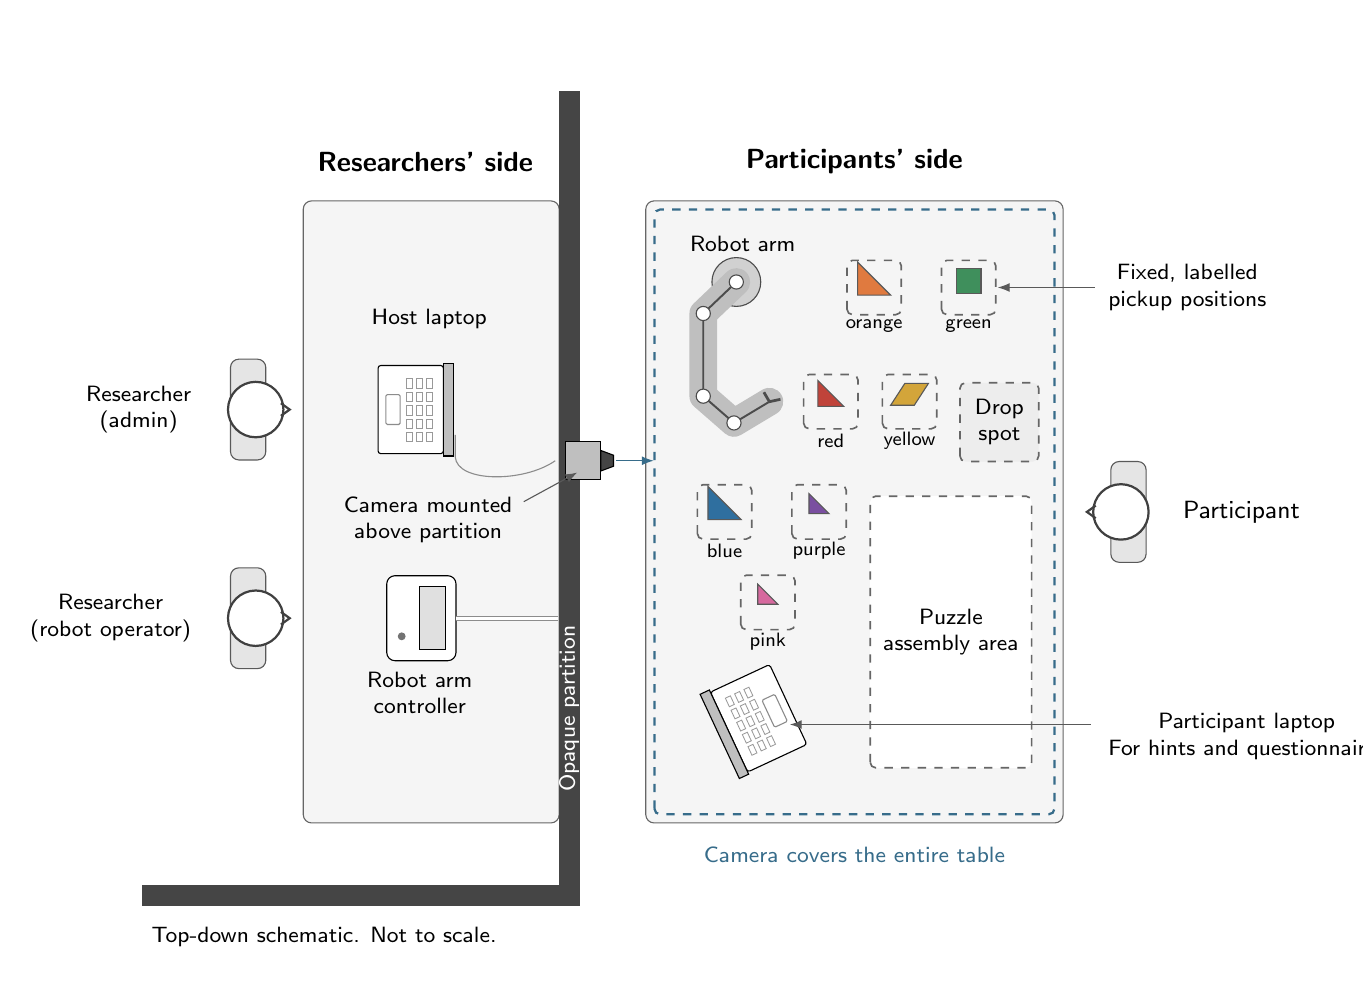
\begin{tikzpicture}[x=1cm,y=1cm,font=\sffamily\small,
  label/.style={align=center},
  leader/.style={-{Latex[length=1.5mm]},thin,draw=black!65},
  zone/.style={draw=black!60,dashed,rounded corners=2pt,line width=.6pt}]
\path[use as bounding box] (-2.8,.1) rectangle (13.8,11.9);

% Two long tables, with the researcher table immediately beside the partition.
\draw[fill=tablefill,draw=black!60,rounded corners=3pt] (.7,1.8) rectangle (3.95,9.7);
\draw[fill=tablefill,draw=black!60,rounded corners=3pt] (5.05,1.8) rectangle (10.35,9.7);
\fill[wallfill] (3.95,.75) rectangle (4.21,11.1);
\fill[wallfill] (-1.35,.75) rectangle (4.21,1.01);
\node[rotate=90,text=white,font=\sffamily\footnotesize] at (4.08,3.25) {Opaque partition};
\node[label,font=\sffamily\bfseries] at (2.25,10.2) {Researchers' side};
\node[label,font=\sffamily\bfseries] at (7.7,10.2) {Participants' side};

% Admin sits to the left; host laptop faces left toward the admin.
\begin{scope}[shift={(2.3,7.05)},rotate=-90]
\planlaptop
\end{scope}
\node[label,font=\sffamily\footnotesize] at (2.3,8.2) {Host laptop};
\draw[black!45] (2.63,6.73) -- (2.63,6.45) .. controls (2.65,6.12) and (3.5,6.12) .. (3.9,6.4);

% Controller faces its operator; connection leads toward the partition.
\draw[fill=white,rounded corners=3pt] (1.76,3.86) rectangle (2.64,4.94);
\draw[fill=black!12] (2.18,4.0) rectangle (2.51,4.8);
\fill[black!55] (1.95,4.17) circle (.05);
\draw[black!45,double,double distance=1pt] (2.64,4.4) -- (3.93,4.4);
\node[label,font=\sffamily\footnotesize] at (2.18,3.45) {Robot arm\\controller};

% Plan-view heads and shoulders face the tables, rather than the page bottom.
\foreach \yy in {7.05,4.4} {
  \begin{scope}[shift={(0,\yy)},scale=1.6]
    \draw[fill=black!10,draw=black!65,rounded corners=3pt] (-.14,-.4) rectangle (.14,.4);
    \draw[fill=white,draw=black!75,line width=.8pt] (.06,0) circle (.22);
    \draw[black!75,line width=.8pt] (.26,.05) -- (.33,0) -- (.26,-.05);
  \end{scope}
}
\node[label,anchor=east,font=\sffamily\footnotesize] at (-.6,7.05) {Researcher\\(admin)};
\node[label,anchor=east,font=\sffamily\footnotesize] at (-.6,4.4) {Researcher\\(robot operator)};
\begin{scope}[shift={(11.18,5.75)},xscale=-1.6,yscale=1.6]
  \draw[fill=black!10,draw=black!65,rounded corners=3pt] (-.14,-.4) rectangle (.14,.4);
  \draw[fill=white,draw=black!75,line width=.8pt] (.06,0) circle (.22);
  \draw[black!75,line width=.8pt] (.26,.05) -- (.33,0) -- (.26,-.05);
\end{scope}
\node[label,anchor=west] at (11.75,5.75) {Participant};

% Camera centred on the partition in plan view; mounted above it.
\draw[fill=black!25] (4.03,6.16) rectangle (4.48,6.64);
\draw[fill=wallfill] (4.48,6.27) -- (4.64,6.33) -- (4.64,6.47) -- (4.48,6.53) -- cycle;
\node[label,anchor=east,font=\sffamily\footnotesize] at (3.48,5.65) {Camera mounted\\above partition};
\draw[leader] (3.5,5.88) -- (4.18,6.25);
\draw[viewblue,dashed,line width=.8pt,rounded corners=2pt] (5.16,1.91) rectangle (10.24,9.59);
\draw[leader,viewblue] (4.67,6.4) -- (5.15,6.4);
\node[label,text=viewblue,font=\sffamily\footnotesize] at (7.7,1.4) {Camera covers the entire table};

% Bent arm in the upper-left corner, following the sketch's orientation.
\begin{scope}[yshift=-.3cm]
\draw[fill=black!18,draw=black!70] (6.2,8.97) circle (.31);
\draw[black!25,line width=10pt,line cap=round,line join=round]
  (6.2,8.97) -- (5.78,8.57) -- (5.78,7.52) -- (6.17,7.18) -- (6.62,7.45);
\draw[black!70,line width=.7pt]
  (6.2,8.97) -- (5.78,8.57) -- (5.78,7.52) -- (6.17,7.18) -- (6.62,7.45);
\foreach \pos in {(6.2,8.97),(5.78,8.57),(5.78,7.52),(6.17,7.18)}
  \draw[fill=white,draw=black!70] \pos circle (.09);
\draw[black!70,line width=1pt] (6.55,7.57) -- (6.62,7.45) -- (6.76,7.48);
\node[label,font=\sffamily\footnotesize] at (6.28,9.45) {Robot arm};
\end{scope}

% Seven pickup positions follow the table sketch: two, two, two, then one.
% Exact colour-to-position mapping awaits confirmation against the real setup.
\foreach \xx/\yy in {7.95/8.6,9.15/8.6,8.4/7.15,7.4/7.15,6.6/4.6,7.25/5.75,6.05/5.75} {
  \draw[zone] (\xx-.345,\yy-.345) rectangle (\xx+.345,\yy+.345);
}
\begin{scope}[shift={(7.95,8.6)},scale=.75]
  \filldraw[fill=pieceorange,draw=black!65] (-.28,-.13) -- (.28,-.13) -- (-.28,.43) -- cycle;
  \node[font=\sffamily\scriptsize] at (0,-.66) {orange};
\end{scope}
\begin{scope}[shift={(9.15,8.6)},scale=.75]
  \filldraw[fill=piecegreen,draw=black!65] (-.21,-.1) rectangle (.21,.32);
  \node[font=\sffamily\scriptsize] at (0,-.66) {green};
\end{scope}
\begin{scope}[shift={(8.4,7.15)},scale=.75]
  \filldraw[fill=pieceyellow,draw=black!65] (-.32,-.06) -- (.08,-.06) -- (.32,.31) -- (-.08,.31) -- cycle;
  \node[font=\sffamily\scriptsize] at (0,-.66) {yellow};
\end{scope}
\begin{scope}[shift={(7.4,7.15)},scale=.75]
  \filldraw[fill=piecered,draw=black!65] (-.22,-.08) -- (.22,-.08) -- (-.22,.36) -- cycle;
  \node[font=\sffamily\scriptsize] at (0,-.66) {red};
\end{scope}
\begin{scope}[shift={(6.6,4.6)},scale=.75]
  \filldraw[fill=piecepink,draw=black!65] (-.17,-.03) -- (.17,-.03) -- (-.17,.31) -- cycle;
  \node[font=\sffamily\scriptsize] at (0,-.66) {pink};
\end{scope}
\begin{scope}[shift={(7.25,5.75)},scale=.75]
  \filldraw[fill=piecepurple,draw=black!65] (-.17,-.03) -- (.17,-.03) -- (-.17,.31) -- cycle;
  \node[font=\sffamily\scriptsize] at (0,-.66) {purple};
\end{scope}
\begin{scope}[shift={(6.05,5.75)},scale=.75]
  \filldraw[fill=pieceblue,draw=black!65] (-.28,-.13) -- (.28,-.13) -- (-.28,.43) -- cycle;
  \node[font=\sffamily\scriptsize] at (0,-.66) {blue};
\end{scope}
\node[label,anchor=west,font=\sffamily\footnotesize] at (10.8,8.6) {Fixed, labelled\\pickup positions};
\draw[leader] (10.75,8.6) -- (9.52,8.6);

% Participant faces page-left: their right is page-up and left is page-down.
% Tall solving area at lower right; drop spot directly above, as in the table sketch.
\draw[zone,fill=white] (7.9,2.5) rectangle (9.95,5.95);
\node[label,font=\sffamily\footnotesize] at (8.925,4.225) {Puzzle\\assembly area};
\draw[zone,fill=black!7] (9.04,6.39) rectangle (10.04,7.39);
\node[label,font=\sffamily\footnotesize] at (9.54,6.89) {Drop\\spot};

% Participant laptop at the lower-left, angled toward the participant on the right.
\begin{scope}[shift={(6.27,3.03)},rotate=115]
\planlaptop
\end{scope}
\node[label,anchor=west,font=\sffamily\footnotesize] at (10.8,2.9) {Participant laptop\\For hints and questionnaires};
\draw[leader] (10.7,3.05) -- (6.88,3.05);
\node[label,font=\sffamily\footnotesize,anchor=west] at (-1.35,.35) {Top-down schematic. Not to scale.};
\end{tikzpicture}
\end{document}
